\documentclass{article}
\usepackage[utf8]{inputenc}
\usepackage{amsmath, graphicx}
\usepackage[]{algorithm2e}
\usepackage[margin=1in]{geometry}

\allowdisplaybreaks

\makeatletter
\renewcommand\thesection{}
\renewcommand\thesubsection{\@arabic\c@section.\@arabic\c@subsection}
\makeatother

\title{\vspace{-5ex}Random Graphs Project 4}
\author{Alex Rose, Pedro Rodriguez}
\date{April 2016}

\begin{document}

\maketitle
\vspace{-15ex}
\section{}
\subsection{ }
\vspace{-2ex}
$$P(E_n) = pP(E_{n-1}) + (1-p)P(\neg E_{n-1}) = pP(E_{n-1}) + (1-p)(1- P(E_{n-1}) $$
$$ = (2p-1)P(E_{n-1}) + (1 - p), P(E_0) = p$$
\vspace{-6ex}
\subsection{} 
\vspace{-2ex}
$$
\begin{aligned}
P(E_n)&=f(n)=(2p-1)f(n-1)+1-p\\
r&=2p-1&\text{Characteristic function}\\
f_g(n)&=a(2p-1)^n&\text{General solution}\\
f(n)&=c=(2p-1)c+1-p=2pc-c+1-p=\frac{1}{2}\\
f(n)&=a(2p-a)^n+\frac{1}{2}\\
f(0)&=p=1+\frac{1}{2},a=p-\frac{1}{2}\\
f(n)&=P(E_n)=(p-1/2)(2p-1)^n+\frac{1}{2}
\end{aligned}
$$
Since $0<p<1$, $2p<2$ which implies that $2p-1<1$. From there we see $\lim_{n\rightarrow\infty}(p-1/2)(2p-1)^n+\frac{1}{2}=\frac{1}{2}$

\vspace{-2ex}
\subsection{}
\vspace{-2ex}
Each step of the process removes 2 "degrees" from the degree list to form 1 edge. We have D degrees, so this process will form $D/2$ edges in total.
\vspace{-2ex}
\subsection{}
\vspace{-2ex}
%I'm unhappy with this section. I provide a counterexample, but no actual insight on why the two SHOULD be different. 
 The procedures are \textit{not} equivalent. Consider a three node graph with a Bernoulli fixed degree distribution, with probability $p$ that the node has degree 0 and probability $1-p$ it has degree 1.  Consider the probabilities of each procedure generating a graph with no edges: \\
 
 \textbf{First procedure}: By construction, $P(000| E)$ is the probability the first procedure generates the unordered degree list $(0,0,0)$. By Bayes Theorem we have:
 
 $$P(000|E) = \frac{P(E|000)P(000)}{P(E)}$$
 
 $P(E)$ is given by the sum of the even degree probabilities, $P(000)$ and $011$, so:
 
 $$P(000|E) = \frac{P(000)}{P(000) + P(011)} = \frac{p^3}{p^3 + \binom{3}{1}p(1-p)^2} = \frac{p^3}{p^3 + 3p(1-p)^2}$$
 
 \textbf{Second Procedure}: This procedure freely generates two degrees, and then forces the third degree to make the sum of all three degrees even. Note the only way to generate 000 is to have the two free values be 00. If that happens, then the third value must be 0 to preserve eveness. And so the probability of the second procedure generating (000) is the probability it generates the free degrees 00, which is $p^2$. \\
 
 $p^2$ is not uniformly equal to $\frac{p^3}{p^3 + 3p(1-p)^2}$ on $0 < p < 1$, and so the two procedures are not equivalent.

\vspace{-2ex}
\subsection{} 
\vspace{-2ex}
\begin{algorithm}[H]
 Degrees = None, Edges = NxN Matrix\;
 \While{Degrees is None}{
 Vec = create N length vector with N draws from simulate(d)\;
  \If{sum of Vec is even}{
	Degrees = Vec\;
   }
 }
half\_edges = create a list with Degrees[i] instances of i\;
random.shuffle(half\_edges)\;
\While{len(half\_edges) above 0}{
	u, v = pop(half\_edges), pop(half\_edges\;
	\If{u == v}{
	Edges[u, v] += 1
	}
	\Else{
	Edges[u,v] += 1
	Edges[v,u] += 1
	}
 }
\Return Edges

\end{algorithm}

\subsection{}
\vspace{-2ex}
Let $S_t = d_1 + d_2 + ... + d_t$. Then:

$$q_n  = \begin{cases}
  P(E_{n-t}), & \text{if } S \text{ is even}, \\
  1 - P(E_{n-t}), & \text{if }  S \text{ is odd}.
\end{cases}$$

As $t$ is finite, we have:
$$\lim_{n\to\infty} P(E_{n-t}) = \lim_{n\to\infty} P(E_{n})  = 1/2$$. 

So $\lim_{n\to\infty} q_n = 1/2$ in both cases.

\subsection{}
\vspace{-2ex}
Let $D_t$ denote event $(d_1 = k_1, d_2 = k_2,..., d_t = k_t)$. By Baye's Theorem:

$$ \lim_{n\to\infty} P(D_t | E_n) = \lim_{n\to\infty} \frac{P(E_n | D_t)P(D_t)}{P(E_n)} = \frac{1/2* P(D_t)}{1/2} = P(D_t) $$

And the variables $d_1...d_n$ are all independent by assumption, so:
$$P(D_t) = P(d_1 = k_1) P(d_2 = k_2) ... P(d_t = k_t) = \prod_{j=1}^{t} P(d_j)$$ 

\newpage
\section{}
\subsection{}
$$
\begin{aligned}
&d\sim Binomial(n,p),n=5,p=1/2\\
\mu_1&=E[d]=np\\
E[d^2]&=Var(d)+E[d]^2=np(1-p)+n^2p^2=np-np^2+n^2p^2\\
\mu_2&=E[d^2]-E[d]=np-np^2+n^2p^2-np=n^2p^2-np^2\\
\frac{\mu_2}{2\mu_1}&=\frac{n^2p^2-np^2}{2np}=\frac{np-p}{2}=1=(\frac{\mu_2}{2\mu_1})^2
\end{aligned}
$$

$$
\begin{aligned}
&d\sim Geometric(p),p=2/5\\
\mu_1&=E[d]=\frac{1}{p}\\
E[d^2]&=Var(d)+E[d]^2=\frac{1-p}{p^2}+\frac{1}{p^2}\\
\mu_2&=E[d^2]-E[d]=\frac{1-p}{p^2}+\frac{1}{p^2}-\frac{1}{p}=\frac{2-2p}{p^2}\\
\frac{\mu_2}{2\mu_1}&=\frac{2-2p}{2p^2}\cdot p=\frac{1-p}{p}=1.5\\
(\frac{\mu_2}{2\mu_1})^2&=2.25
\end{aligned}
$$

For all experiments, $n=250$.

The results show that for the binomial we wish to compare against $Poisson(1)$ and geometric against $Poisson(1.5)$. Experimental results are shown in figure \ref{loop}. The plots agree well with theoretical results.

\begin{figure}[!ht]
	\centering
	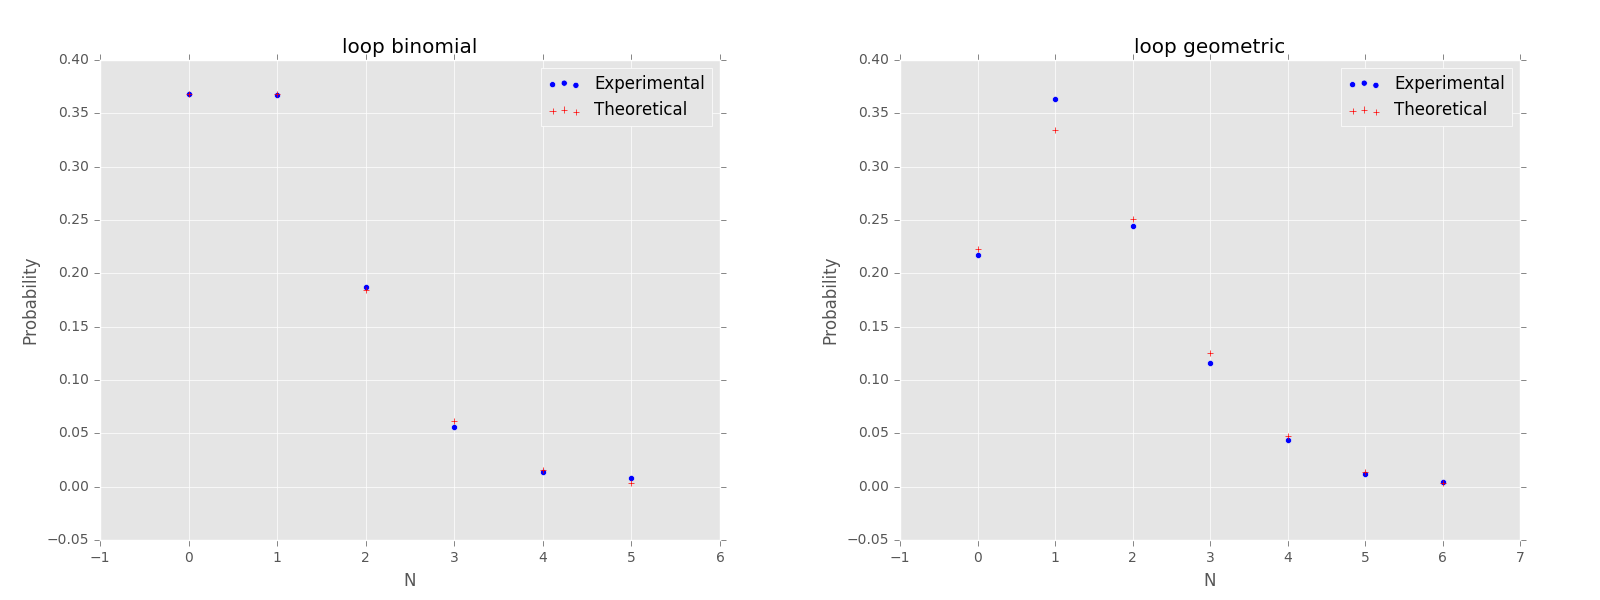
\includegraphics[width=\textwidth]{loop.png}
	\label{loop}
\end{figure}

\subsection{}
\vspace{-2ex}
The results show that for the binomial we wish to compare against $Poisson(1)$ and geometric against $Poisson(2.25)$. Experimental results are shown in figure \ref{parallel}. The plots agree well with theoretical results.

\begin{figure}[!ht]
	\centering
	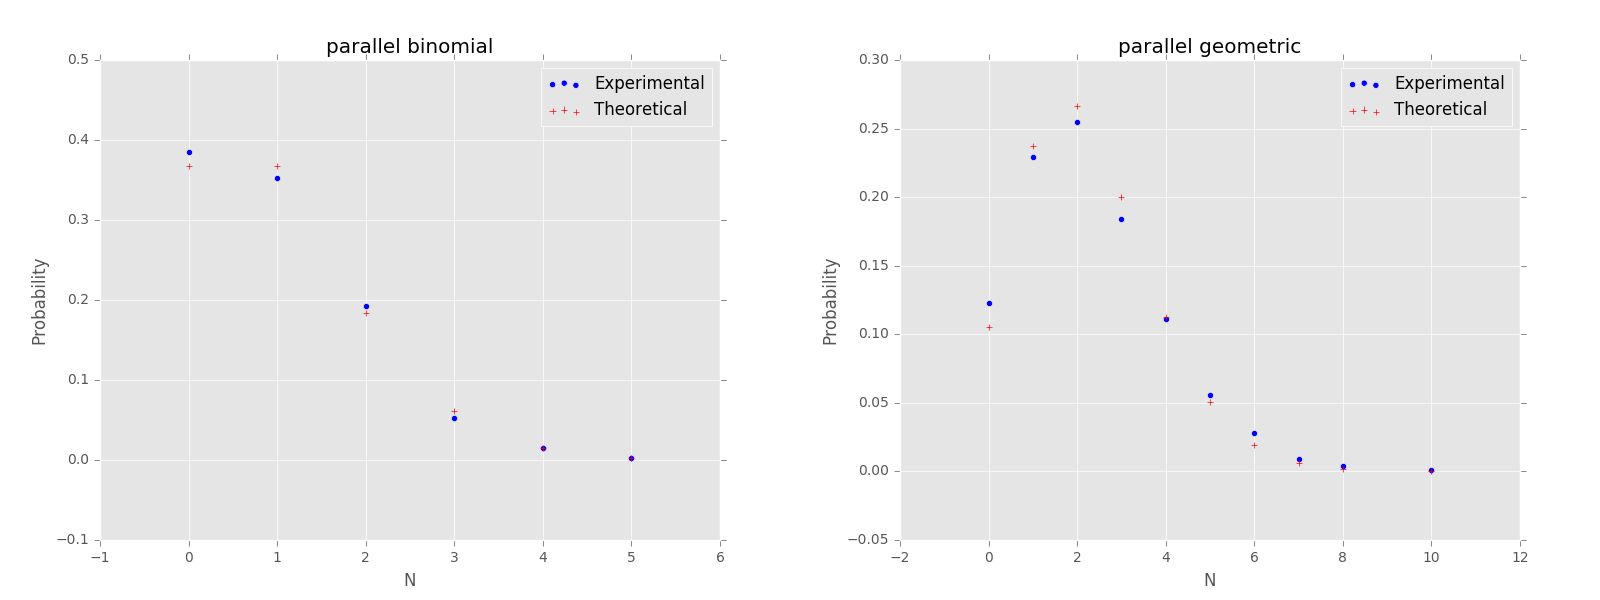
\includegraphics[width=\textwidth]{parallel.png}
	\label{parallel}
\end{figure}

\subsection{}
\vspace{-2ex}
The counts of loops and parallel edges in a simple graph is zero, thus:

For $d\sim Binomial(5,1/2)$, $P(simple)=p_1(0)\cdot p_1(0)=.367^2=.135$. Five experimental runs of 1K graphs yields $[.131,.12,.138,.118,.144]$ which agrees well with the theoretical result.

For $d\sim Geometric(2/5)$, $P(simple)=p_{1.5}(0)\cdot p_{2.25}(0)=.0235$. Five experimental runs of 1K graphs yields $[.03,.026,.03, .025, .023]$. These results generally agree, but not that the mean of the runs is slightly high. To alleviate this, a higher $n$ may help, but was difficult because counting parallel edges in our algorithm is $O(n^2)$ and took a long time to ran for anything significantly above $n=250$.

\end{document}
